% Also note that the "draftcls" or "draftclsnofoot", not "draft", option
% should be used if it is desired that the figures are to be displayed in
% draft mode.
%
\documentclass[conference]{IEEEtran}
% Add the compsoc option for Computer Society conferences.

% Some very useful LaTeX packages include:
% (uncomment the ones you want to load)

\usepackage{cite}
\ifCLASSINFOpdf
   \usepackage[pdftex]{graphicx}
  % declare the path(s) where your graphic files are
   \graphicspath{{Images/}}
  % and their extensions so you won't have to specify these with
  % every instance of \includegraphics
   \DeclareGraphicsExtensions{.pdf,.jpeg,.png}
\else
  % or other class option (dvipsone, dvipdf, if not using dvips). graphicx
  % will default to the driver specified in the system graphics.cfg if no
  % driver is specified.
  % \usepackage[dvips]{graphicx}
  % declare the path(s) where your graphic files are
  % \graphicspath{{../eps/}}
  % and their extensions so you won't have to specify these with
  % every instance of \includegraphics
  % \DeclareGraphicsExtensions{.eps}
\fi
% graphicx was written by David Carlisle and Sebastian Rahtz. It is
% required if you want graphics, photos, etc. graphicx.sty is already
% installed on most LaTeX systems. The latest version and documentation
% can be obtained at: 
% http://www.ctan.org/tex-archive/macros/latex/required/graphics/
% Another good source of documentation is "Using Imported Graphics in
% LaTeX2e" by Keith Reckdahl which can be found at:
% http://www.ctan.org/tex-archive/info/epslatex/
%
% latex, and pdflatex in dvi mode, support graphics in encapsulated
% postscript (.eps) format. pdflatex in pdf mode supports graphics
% in .pdf, .jpeg, .png and .mps (metapost) formats. Users should ensure
% that all non-photo figures use a vector format (.eps, .pdf, .mps) and
% not a bitmapped formats (.jpeg, .png). IEEE frowns on bitmapped formats
% which can result in "jaggedy"/blurry rendering of lines and letters as
% well as large increases in file sizes.
%
% You can find documentation about the pdfTeX application at:
% http://www.tug.org/applications/pdftex


% correct bad hyphenation here
\hyphenation{op-tical net-works semi-conduc-tor}

\usepackage{url}
\usepackage[table, svgnames]{xcolor} 
\usepackage{color}

\begin{document}
%
% paper title
% can use linebreaks \\ within to get better formatting as desired
% Do not put math or special symbols in the title.
\title{Security-Related Questions Developers Ask About Their Code}


% author names and affiliations
% use a multiple column layout for up to three different
% affiliations
\author{\IEEEauthorblockN{Justin Smith, Brittany Johnson, and Emerson Murphy-Hill}
\IEEEauthorblockA{North Carolina State University\\
Raleigh, North Carolina}}


% conference papers do not typically use \thanks and this command
% is locked out in conference mode. If really needed, such as for
% the acknowledgment of grants, issue a \IEEEoverridecommandlockouts
% after \documentclass

\maketitle

% As a general rule, do not put math, special symbols or citations
% in the abstract
\begin{abstract}

New tools and approaches should help developers answer the security-relevant questions that they would otherwise struggle with. 
To design tools that help developers answer their questions, we must first understand what questions they ask.
However, we lack a catalog and categorization of such questions. 
Our work identifies the security-related questions developers ask, explores the strategies that developers use to answer those questions, and assesses the existing tool support for those strategies.  
We contribute by informing toolsmiths of the security-related questions that developers ask.

We identified developers' knowledge requirements by conducting 10 semi-structured interviews with novice and experienced software developers, observing their interactions with security vulnerabilities in iTrust, a Java medical records software system.
From these interactions, we extracted 559 questions, which we reduced to 155 unique questions that fit into 17 categories.


\end{abstract}
% no keywords

% For peer review papers, you can put extra information on the cover
% page as needed:
% \ifCLASSOPTIONpeerreview
% \begin{center} \bfseries EDICS Category: 3-BBND \end{center}
% \fi
%
% For peerreview papers, this IEEEtran command inserts a page break and
% creates the second title. It will be ignored for other modes.
\IEEEpeerreviewmaketitle



\section{Introduction}
% no \IEEEPARstart

When analyzing source code, especially defective code, research suggests that during this knowledge acquisition process, developers hypothesize about the code, specifically by asking questions~\cite{livshits2005finding, ko2004designing}. 
There exists research that attempts to categorize and catalog the questions developers ask when coding~\cite{latoza2010hard}. 
Research on tool design and developer productivity have used available catalogs to design tools that support developers when attempting to answer these questions~\cite{yoon2013visualization, servant2012history}.

 
Professionals working on security-critical applications also could benefit from improved tool support in their work environments. 
There exist tools that help developers detect potential security flaws in their code. 
However, research suggests they may not be using them because of difficulty interpreting the output~\cite{johnson2013don}. 
Part of this difficulty for security developers may stem from the fact that some of the hard to answer questions developers have pertain to the security of their code~\cite{latoza2010hard}.

%This is a bit redundant but it's all here
Despite the importance of security, to our knowledge, no research exists that catalogs the specific security-related questions developers ask. 
Therefore, we lack a framework for assessing whether existing tools fully address the knowledge requirements of developers.

Research that determines the questions developers ask about their code has informed and motivated toolsmiths in other domains to develop better tools~\cite{kononenko2012automatically, servant2012history, yoon2013visualization}.
Our work extends these promising results to security by informing toolsmiths of the security-related questions that developers ask.
In this paper, we report a study conducted with 10 developers familiar with the iTrust software system.\footnote{\url{http://agile.csc.ncsu.edu/iTrust/wiki/doku.php?id=start}} 
We observed each developer as they assessed potential security vulnerabilities in the code and report the kinds of questions they asked while doing so. Using a card sort methodology, we sorted the 559 questions into 17 categories. 

The main contribution of this paper is categorized questions developers ask. 
We also assess the strategies developers use to answer these questions and whether or not existing tools support these strategies.

The remainder of the paper is organized as follows. 
In Section~\ref{sec:rw}, we discuss previous work related to our own. 
Section~\ref{sec:meth} outlines the methodology we used to conduct our study and analyze our data. 
Next, we discuss the findings of our study in Section~\ref{sec:results} and implications of our findings in Section~\ref{sec:disc}. 
Finally, we conclude the paper with a discussion of future work~\ref{sec:fw}.



% An example of a floating figure using the graphicx package.
% Note that \label must occur AFTER (or within) \caption.
% For figures, \caption should occur after the \includegraphics.
% Note that IEEEtran v1.7 and later has special internal code that
% is designed to preserve the operation of \label within \caption
% even when the captionsoff option is in effect. However, because
% of issues like this, it may be the safest practice to put all your
% \label just after \caption rather than within \caption{}.
%
% Reminder: the "draftcls" or "draftclsnofoot", not "draft", class
% option should be used if it is desired that the figures are to be
% displayed while in draft mode.
%
%\begin{figure}[!t]
%\centering
%\includegraphics[width=2.5in]{myfigure}
% where an .eps filename suffix will be assumed under latex, 
% and a .pdf suffix will be assumed for pdflatex; or what has been declared
% via \DeclareGraphicsExtensions.
%\caption{Simulation Results.}
%\label{fig_sim}
%\end{figure}

% Note that IEEE typically puts floats only at the top, even when this
% results in a large percentage of a column being occupied by floats.


% An example of a double column floating figure using two subfigures.
% (The subfig.sty package must be loaded for this to work.)
% The subfigure \label commands are set within each subfloat command,
% and the \label for the overall figure must come after \caption.
% \hfil is used as a separator to get equal spacing.
% Watch out that the combined width of all the subfigures on a 
% line do not exceed the text width or a line break will occur.
%
%\begin{figure*}[!t]
%\centering
%\subfloat[Case I]{\includegraphics[width=2.5in]{box}%
%\label{fig_first_case}}
%\hfil
%\subfloat[Case II]{\includegraphics[width=2.5in]{box}%
%\label{fig_second_case}}
%\caption{Simulation results.}
%\label{fig_sim}
%\end{figure*}
%
% Note that often IEEE papers with subfigures do not employ subfigure
% captions (using the optional argument to \subfloat[]), but instead will
% reference/describe all of them (a), (b), etc., within the main caption.


% An example of a floating table. Note that, for IEEE style tables, the 
% \caption command should come BEFORE the table. Table text will default to
% \footnotesize as IEEE normally uses this smaller font for tables.
% The \label must come after \caption as always.
%
%\begin{table}[!t]
%% increase table row spacing, adjust to taste
%\renewcommand{\arraystretch}{1.3}
% if using array.sty, it might be a good idea to tweak the value of
% \extrarowheight as needed to properly center the text within the cells
%\caption{An Example of a Table}
%\label{table_example}
%\centering
%% Some packages, such as MDW tools, offer better commands for making tables
%% than the plain LaTeX2e tabular which is used here.
%\begin{tabular}{|c||c|}
%\hline
%One & Two\\
%\hline
%Three & Four\\
%\hline
%\end{tabular}
%\end{table}


%Figure, high res, png or vector (pdf)

\section{Related Work}
\label{sec:rw}

We have organized the related work into three sections. Section \ref{evaluation} outlines the predominant approaches researchers use to evaluate security tools. 
Section \ref{understanding} surveys the work done to facilitate developers' understanding of code, and section \ref{questions} references similar studies that have explored the questions developers ask when modifying, understanding, or debugging their code.

\subsection{Evaluation of Techniques}
\label{evaluation}
Developers use several techniques and tools to help secure their systems.
Using a variety of metrics, many studies have assessed the effectiveness of the tools and techniques developers use to find and remove vulnerabilities from their code~\cite{martin2005finding, austin2011one, livshits2005finding}.  

Much research has evaluated the effectiveness of tools and techniques based on their false positive rates and how many vulnerabilities they detect~\cite{jovanovic2006pixy, austin2011one, dukes2013case}. 
Jovanovic and colleagues attempt to address the problem of vulnerabilities in web applications by implementing and evaluating \textsc{Pixy}, a static analysis tool that detects cross-site scripting vulnerabilities in PHP scripts~\cite{jovanovic2006pixy}. 
They considered their tool effective because of its low false positive rate (50\%) and its ability to find vulnerabilities previously unknown. 
Similarly, Livshits and Lam evaluated their own approach to static analysis for detecting security vulnerabilities; the static analyzers used are created from specifications provided by the user~\cite{livshits2005finding}. 
They also found their tool to be effective because it had a low false positive rate. 

Austin and Williams compared the effectiveness of four existing techniques for discovering security vulnerabilities: systematic and exploratory manual  penetration testing, static analysis, and automated penetration testing~\cite{austin2011one}. 
Comparing the four approaches based on number of vulnerabilities found, false positive rate, and efficiency, they reported that no one technique was capable of discovering every type of vulnerability. 
Dukes and colleagues conducted a case study comparing static analysis and manual testing techniques used to find security vulnerabilities~\cite{dukes2013case}. 
They found that the combination of manual testing and static analysis was most effective, because it found the most vulnerabilities.


These studies use various measures of effectiveness, such as false positive rates or vulnerabilities found by a tool, but none focus on how developers interact with the tool. 
Further, they do not evaluate whether the tools under study answer questions that developer have about the code or vulnerabilities. 
Unlike existing studies, our study explores the questions developers ask when attempting to understand the vulnerabilities in their code.

\subsection{Developer Understanding}
\label{understanding}
In other, non-security domains, research has shifted focus from the technical effectiveness of program analysis tools to usability~\cite{johnson2013don, ayewah2008using, khoo2008path}. 
These studies sought to evaluate how tools communicate information to developers and how a tool can enhance a developer's understanding of the code. 
Such studies examine proposed and existing approaches using various qualitative methods such as interviews and surveys. 

Some research surrounding tool effectiveness shifted focus from technical effectiveness of program analysis tools to usability~\cite{johnson2013don, ayewah2008using, khoo2008path}. 
The goal of these studies was to evaluate how tool designers can help developers cope with existing or proposed approaches, through comparison of proposed and existing approaches and various qualitative methods, such as interviews and surveys.

Ayewah, Pugh, and colleagues conducted a series of interviews and surveys, along with a controlled user study, in an attempt to better understand the practices and needs of developers when using the static analysis tool FindBugs~\cite{ayewah2008report, ayewah2008using}.

Khoo and colleagues focused their efforts on improving the user interface of existing tools by developing and evaluating \textsc{Path Projection}, a user interface toolkit to help developers navigate through and understand the errors in their code~\cite{khoo2008path}.

Johnson and colleagues conducted semi-structured interviews with professional developers to determine the reason developers have for using, and possibly not using, static analysis tools to find defects in their codes~\cite{johnson2013don}. 
Their findings suggest that one of the biggest reasons developers may have for not using tools to analyze their code is difficulty understanding the output provided. 

Layman and colleagues conducted a study with developers to explore the factors developers consider when deciding whether they will fix a defect or not~\cite{layman2007toward}. Based on their findings, they discuss design implications for automated fault detection tools.

These studies discuss the ability of developers to effectively use existing tools and ways to improve them, however, they do not pay due diligence to how developers interpret the reporting of security vulnerabilities. 
It is particularly important to consider security tools and vulnerabilities, because security vulnerabilities are more likely to cause incidents that affect company budgets as well as the end users~\cite{chen2002mops}. 
Research also suggests that some of the harder questions to answer when analyzing code revolve around security and the implications of changes made to the code on security~\cite{latoza2010hard}.  
The goal of our study is to identify the security-related questions developers ask when approaching security vulnerabilities so that tool designers understand the information requirements of security-minded developers.

\subsection{Answering Developer Questions}
\label{questions}
Several studies have explored the knowledge requirements of developers, however few such studies have focused specifically on the knowledge requirements of developers when assessing security vulnerabilities~\cite{begel2014analyze, latoza2010hard, latoza2010developers}.

LaToza and Myers surveyed professional software developers to understand the questions developers ask during their daily coding activities, focusing on the hard to answer questions~\cite{latoza2010hard}. 

Futhermore, after observing developers in a lab study, they discovered that the questions developers ask tend to be questions revolving around searching through the code for target statements, or reachability questions~\cite{latoza2010developers}. 

Ko and Myers developed \textsc{Whyline}, a tool meant to ease the process of debugging code by helping answer ``why did'' and ``why didn't'' questions developers have~\cite{ko2004designing}. They found that developers were able to complete more debugging tasks when using their tool than they could without it.

Fritz and Murphy developed a model and prototype tool to assist developers with answering the questions they want to ask based on interviews they conducted~\cite{fritz2010using}.

%we know finding answers tedious; our study aims to find the questions and ways tool designers can help developers with this process.  

These studies explore the questions developers ask when building and debugging software, however, they do not study the questions developers ask when they have a potential security vulnerability in their code. 
In fact, our work builds on the work of LaToza and Myers, which found that some of the hard-to-answer questions developers have pertain to the implications of code changes on the security of their code. 
Our study discovers the questions developers have about potential code vulnerabilities and discusses the implications of the changes they may make when attempting to resolve them. 

\section{Methodology}
\label{sec:meth}
We conducted 10 semi-structured interviews with software developers. In our analysis, we extracted and categorized the questions developers asked during these interviews. 
Section \ref{rqs} outlines the research questions we sought to answer. 
Section \ref{studyDesign} details how the study was designed and section \ref{dataAnalysis} describes how we preformed data analysis.


\subsection{Research Questions}
\label{rqs}
We want to answer the following research questions:
\begin{itemize}
\item \textbf{RQ1}: What types of security related questions do developers ask?
\item \textbf{RQ2}: How do current tools and approaches support developers in answering these questions?
\end{itemize}

\subsection{Study Design}
\label{studyDesign}
Each interview started with a five-minute briefing section, followed by encounters with four vulnerabilities.
All participants consented to have their session recorded using screen and audio capture software.
Finally, each interview concluded with several demographic and open-ended discussion questions.


\subsubsection{Materials}

\begin{figure}
\centering
\includegraphics[width=3in]{Images/environment.png}
\caption{The environment participants were presented with.}
\label{fig:environment} 
\end{figure}
	

Participants used Eclipse to explore vulnerabilities in iTrust, a Java medical records application that ensures the privacy and security of patient records according to the HIPAA statue.\footnote{\url{hhs.gov/ocr/privacy/}} 
During the briefing session, participants were given time to familiarize themselves with the development environment and ask any questions about the experimental setup.
Participants were equipped with an extended version FindBugs, Find Security Bugs.\footnote{\url{http://h3xstream.github.io/find-sec-bugs/}} 
We chose Find Security Bugs as a representative tool by comparing the available source code analysis tools listed by NIST, OWASP, and WASC.
Figure \ref{fig:environment} depicts the configuration of the IDE for one of the tasks.



\begin{table*} 
\centering
\caption{Demographics of study participants}
\begin{tabular}{|l|l|c|c|}
\rowcolor{gray!50}
\hline
    Participant			& Job Title 						& Security Vulnerability Familiarity 					& Programming Experience (years) \\
    \hline
    P1			    	& Student     			& 2.5/5												 	&  4.5    \\
    \hline
    P2			    	& Test Engineer    			& 3/5									    			&  8 		\\
    \hline
    P3 					& Development Tester       			& 2/5													&  6 	    	\\
    \hline
    P4					& Software Developer     			& 2/5				 									&  6     	\\
    \hline
    P5					& Student      			& 4/5													&  10 	\\
    \hline
    P6					& Student		    				& 1/5							    					& 4		\\
    \hline
    P7					& Front-end Software Developer    	& 4/5													& 4.5              \\
    \hline
    P8					& Student	    		& 3/5													& 7   \\
    \hline
    P9					& Software Consultant   	 		& 3/5													& 5	  		 \\
    \hline
    P10			    	& Student    			& 3/5										 			& 8	              \\
    \hline
\end{tabular}
\label{table:participants}
\end{table*}



\subsubsection{Participants}

We interviewed a total of 10 software developers, 6 students and 4 professionals. 
All interviews were conducted in-person.
We recruited participants from personal contacts and class rosters, using snowball sampling to find additional qualified participants.
Since extracting data from each interview required intensive analysis, we ceased recruitment when we felt that few new questions were emerging from each additional interview.

To simulate a more realistic work environment, participants were required to have significant experience working on the iTrust code base. 
All participants either completed or served as teaching assistants for a semester-long software engineering course that focused on developing iTrust.

Table~\ref{table:participants} gives additional demographic information on each of the 10 participants. 
Since the focus of our study was to identify the questions developers ask independent of their background, we report on demographic information to ensure a degree of diversity in our sample and contextualize participant's responses.

\subsubsection{Tasks}
Each participant approached four vulnerabilities. 
We presented each participant with this number of vulnerabilities, because in preliminary pilot interviews, participants spent approximately 10-15 minutes with each vulnerability and showed signs of fatigue after 60 minutes.

FindBugs and Find Security Bugs group similar error messages using a system of tags. For example the Null Pointer tag (NP) applies to notifications that warn about the misuse of null. 
To cover a broader set of question topics, we selected vulnerabilities with four different tags.
Find Security Bugs identified three types of naturally occurring vulnerabilities: cross site scripting, path traversal, and predictable random vulnerabilities.
We inserted a SQL injection vulnerability by making minimal modifications to one of the database access objects.
Our modifications preserved the functionality of the original code and were based on examples of SQL injection presented by OWASP.
Table \ref{table:vulnerabilities} summarizes each of the four vulnerabilities. 

\begin{table*} 
\centering
\caption{Four vulnerability exploration tasks}
\begin{tabular}{|l|l|l|l|}
\rowcolor{gray!50}
\hline
    Vulnerability				& Short Description													& Tool's Rank 						& Tool's Confidence\\
    \hline	
    Potential Path Traversal	& An instance of java.io.File is created to read a file.     			& ``Scary''							 	&  Normal\\
    \hline
    Predictable Random			& Use of java.util.Random is predictable. 								& ``Scary''								&  Normal\\
    \hline
    Servlet Parameter 			& The method getParameter returns a String value that is controlled by the client.			& ``Troubling''		&  Low\\
    \hline
    SQL Injection				& [Method name] passes a non-constant String to an execute method on an SQL statement.     	& ``Of Concern''		&  Low\\
    \hline
\end{tabular}
\label{table:vulnerabilities}
\end{table*}

During the briefing section, participants were told that they were in charge of security for iTrust and to approach the vulnerabilities as if they were in their normal work environment.
Additionally, we asked them to use a think aloud protocol. Specifically, they were asked to, ``Say any questions or thoughts that cross your mind regardless of how relevant you think they are.''

The interviewer was equipped with the following questions, but had the freedom to omit questions or ask follow-up questions based on the participant's responses.
\begin{itemize}
\item What are you exploring/trying to figure out right now?
\item What information do you need to proceed?
\item Can you explain what this warning is trying to tell you?
\item Based on your understanding of this error message, what is the percentage likelihood you would modify this section of he code?
\item How would you fix the problem? Where would you start?
\item On a scale of 1-5, how confident are you in your understanding of the error message?
\item On a scale of 1-5, how confident are you that you are making the correct judgments?
\item What information would you like to see added to the error message?
\item What part of the message is most helpful?
\item Look at the error message one last time. Is there any information you initially disregarded?
\item Would you like to share any other thoughts about this vulnerability?
\end{itemize}

\subsection{Data Analysis}
\label{dataAnalysis}
We analyzed interview data using a grounded theory approach~\cite{glaser2009discovery}. 
First, we transcribed all the audio-video files using oTranscribe.\footnote{\url{otranscribe.com}}
Each transcript, along with the associated recording, was analyzed by two of the authors for implicit and explicit questions. 
We also extracted demographic information, self-efficacy scores and whether or not the participant would modify the code. 
The two question sets for each interview were then iteratively compared against each other until the authors reached agreement on the question sets. 
In the remainder of this section, we will detail the question extraction process and question sorting processes, including the criteria used to determine which statements qualified as questions.
\subsubsection{Question Criteria}
Participants ask both explicit and implicit questions. 
Drawing from previous work on utterance interpretation, we developed 5 criteria to assist in the uniform classification of participant statements~\cite{letovsky1987cognitive}. 
A statement was coded as a question only if it met one of the following criteria:

\begin{itemize}
\item \textbf{The participant explicitly asks a question.}
\\ P2: \textit{Why aren't they using Prepared Statements?}
\item \textbf{The participant makes a statement and explores the validity of that statement.}
\\ P6: \textit{It doesn't seem to have shown what I was looking for. Oh, wait! It's right above it...}
\item \textbf{The participant uses key words such as, ``I assume,'' ``I guess,'' or ``I don't know.''}
\\ P8: \textit{I don't know that it's a problem yet.}
\item \textbf{The participant clearly expresses uncertainty over a statement.}
\\ P10: \textit{Well, it's private to this object, right?}
\item \textbf{The participant clearly expresses a knowledge requirement by describing plans to acquire information.}
\\ P1: \textit{I would figure out where it is being called.}

\end{itemize}

\subsubsection{Question Extraction}
Using the criteria outlined in the previous section, each interview was independently coded for questions by two of the authors. 
When we identified a statement that satisfied one or more of the criteria, we marked the transcript, highlighting the participants original statement, and clarified the question being asked.

To handle instances where the two coders disagreed, each interview was reviewed a second time by the two authors that initially coded it.
During the second review, the two reviewers examined each question statement, discussing the justification for each question based on the previously stated criteria.
If one of the reviewers did not agree that a question met at least one of the criteria, the question was removed from the question set. 
When reviewers did agree, they determined the phrasing for the question that was most strongly grounded in the interview artifacts. 
Depending on the participant, inter-reviewer agreement ranged from 91\% to 100\%. Across all participants, agreement averaged to 95\%.

Figure \ref{fig:merging} depicts a section of the questions extracted by both authors from P8 prior to review.

\begin{figure*}
\centering
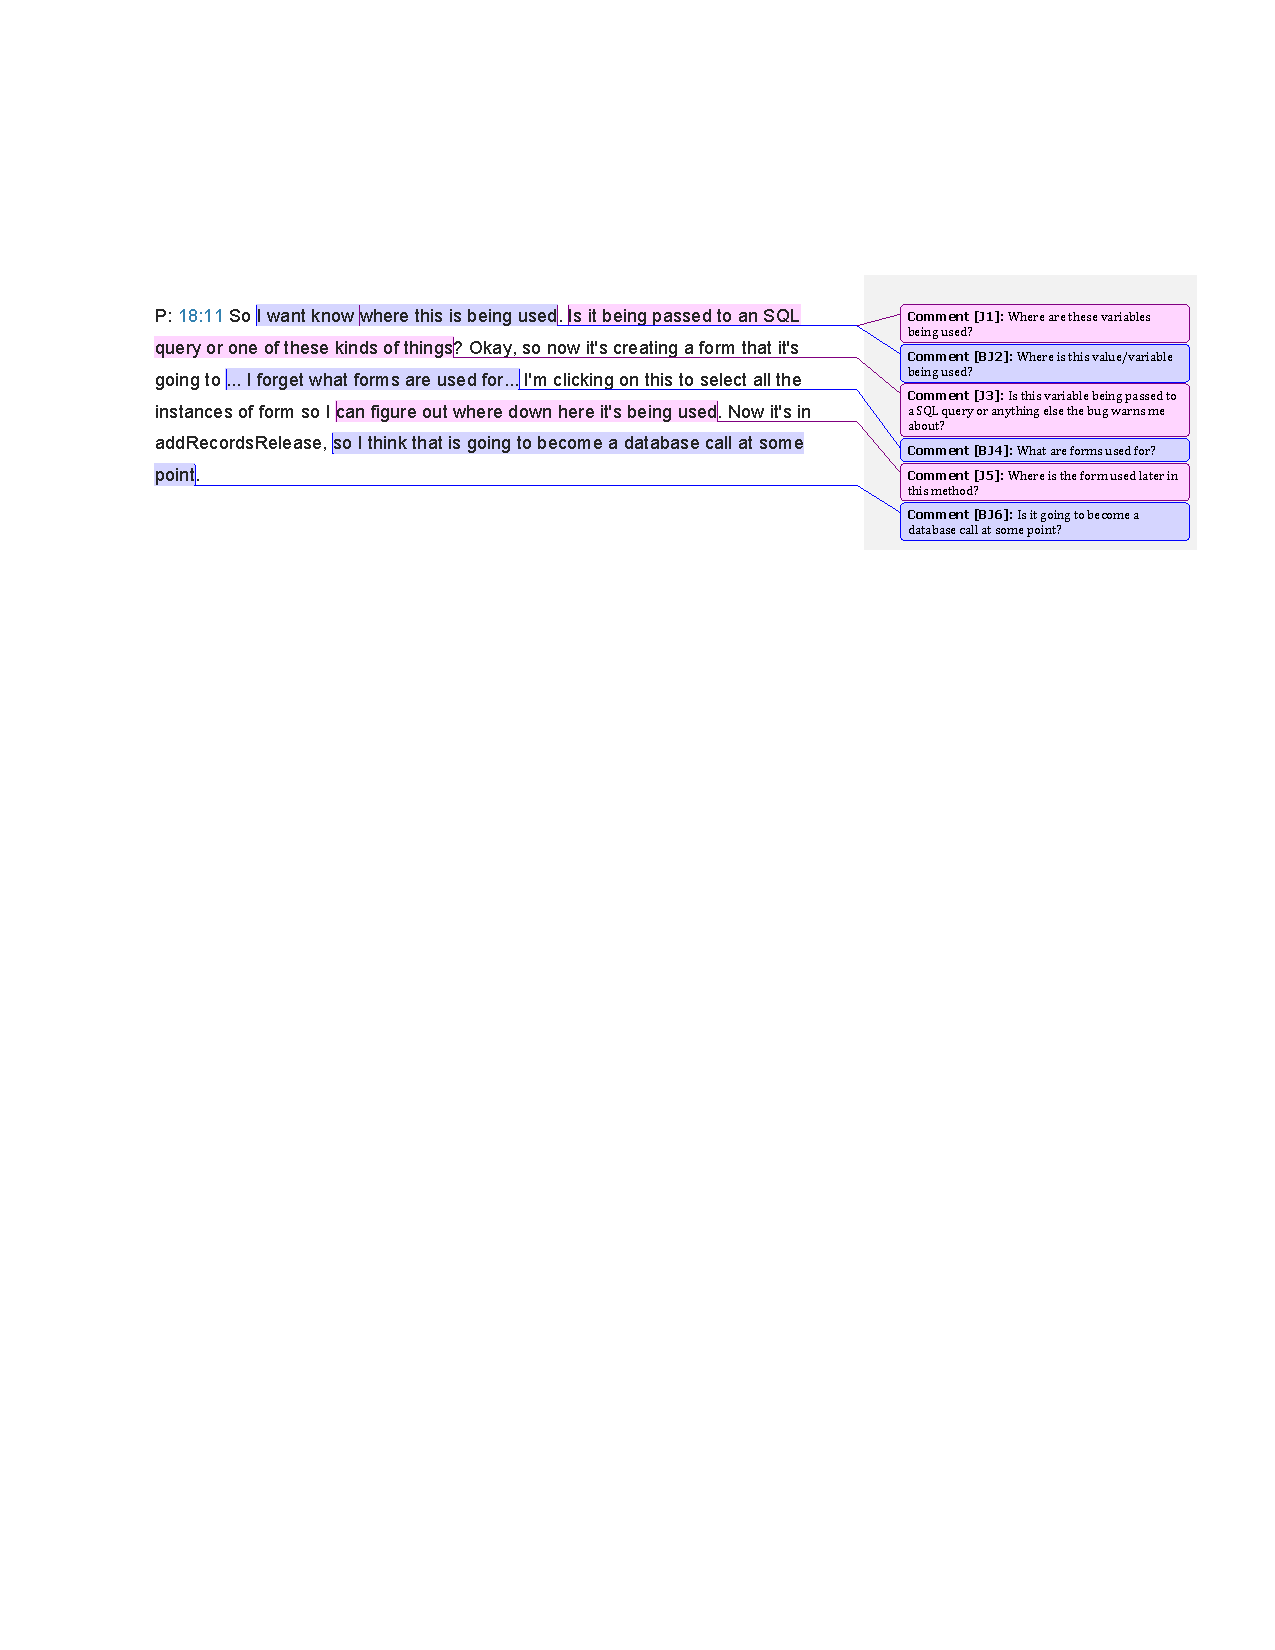
\includegraphics[width=7.5in]{Images/QuestionMerging}
\caption{Question merging process}
\label{fig:merging} 
\end{figure*}

\subsubsection{Question Sorting}
To organize our questions and facilitate discussion, we preformed an \textit{open} card sort~\cite{hudson2013sorting}. 
Card sorting is typically used to help structure data by grouping related information into categories. 
In an \textit{open} sort, the process begins with no notion of predefined categories. 
Rather, sorters derive categories from emergent themes in the cards. 

\begin{figure}
\centering
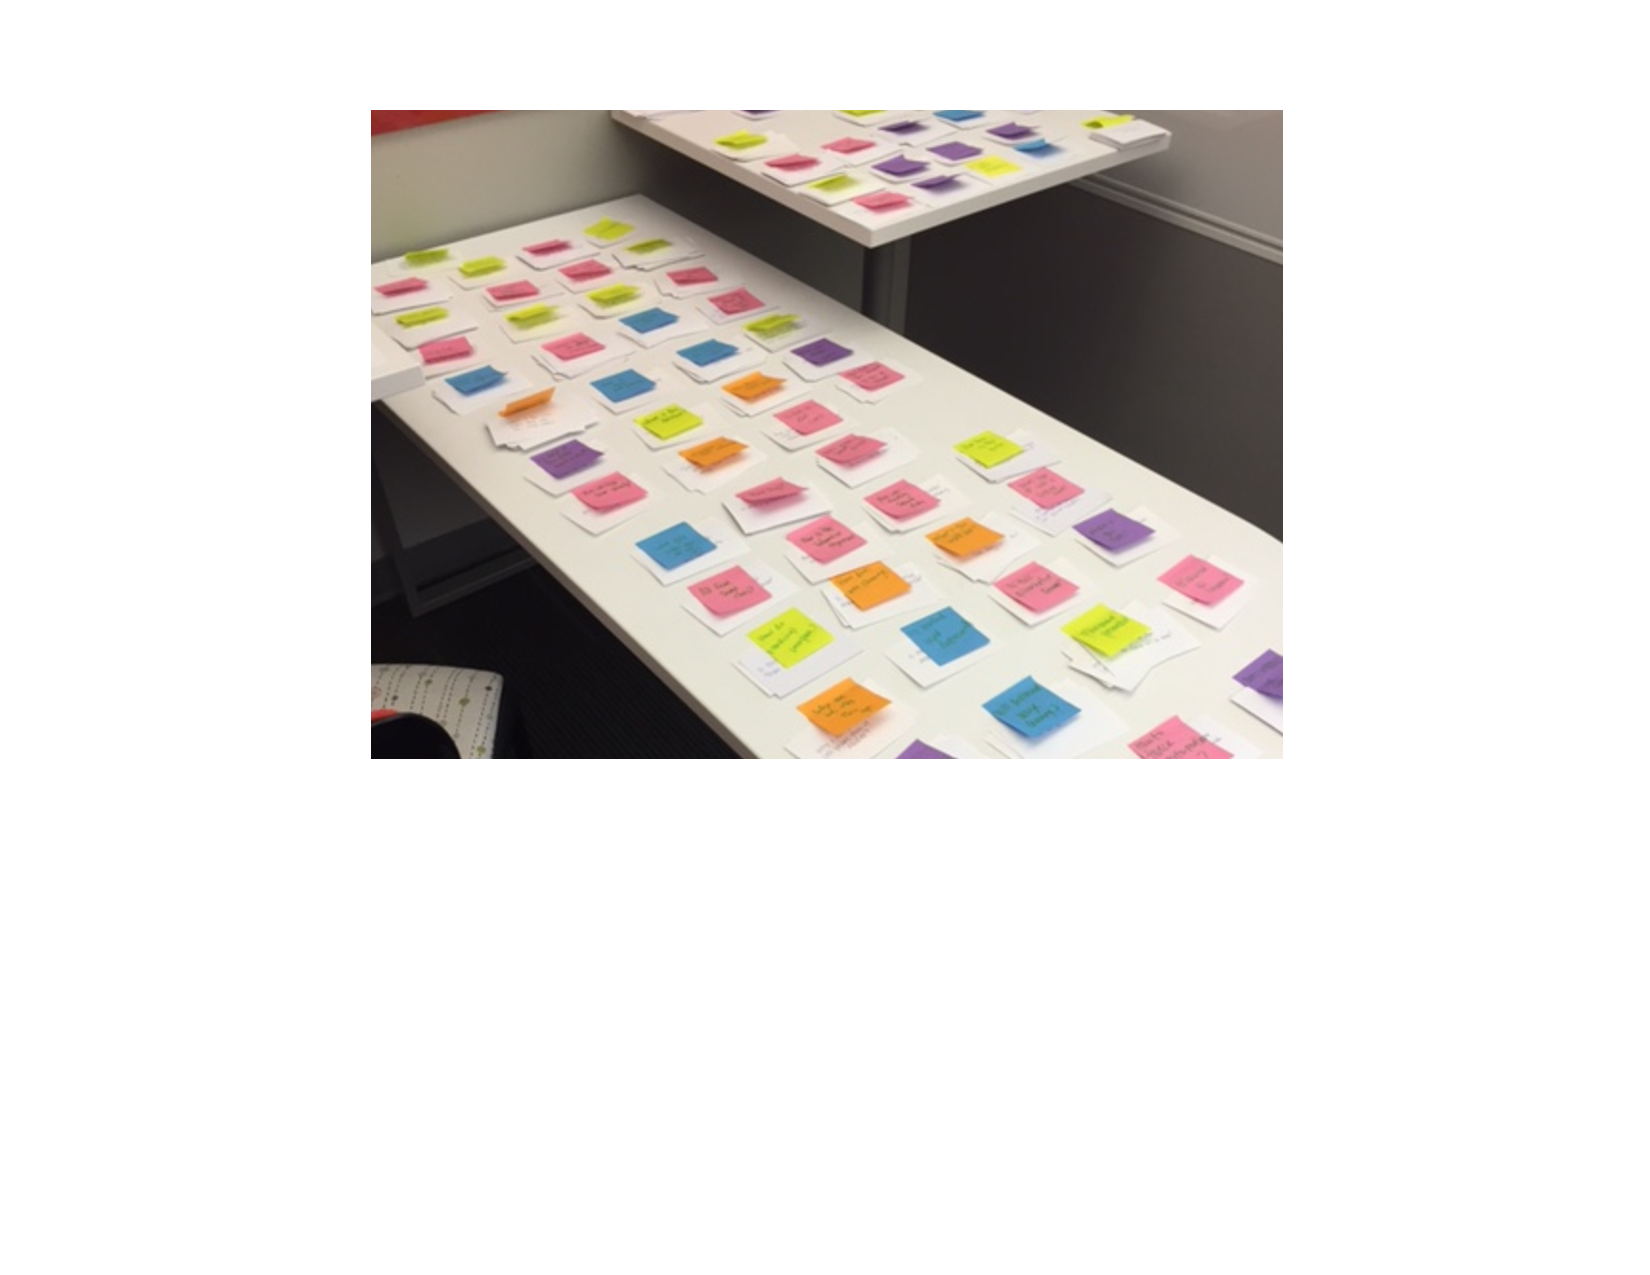
\includegraphics[width=3in]{Images/notecards.pdf}
\caption{Result of phase one of card sorting.}
\label{fig:stageOne} 
\end{figure}

We preformed our card sort in three distinct stages: clustering, categorization, and validation.
 
In the first stage, we formed question clusters by grouping questions that identified the same information requirements (Figure~\ref{fig:stageOne}). 
In this phase we focused on phrasing similar questions consistently and grouping duplicates.
For example, P1 asked, \textit{Where can I find information related to this vulnerability?} P7 asked, \textit{Where can I find an example of using prepared statements?} and P2 asked, \textit{Where can I get more information on path traversal?} 
Of these questions, we created a question cluster labeled \textit{Where can I get more information?}
At this stage, we discarded 5 unclear or non pertinent questions and organized the remaining 554 into 155 unique question clusters.

\begin{figure}
\centering
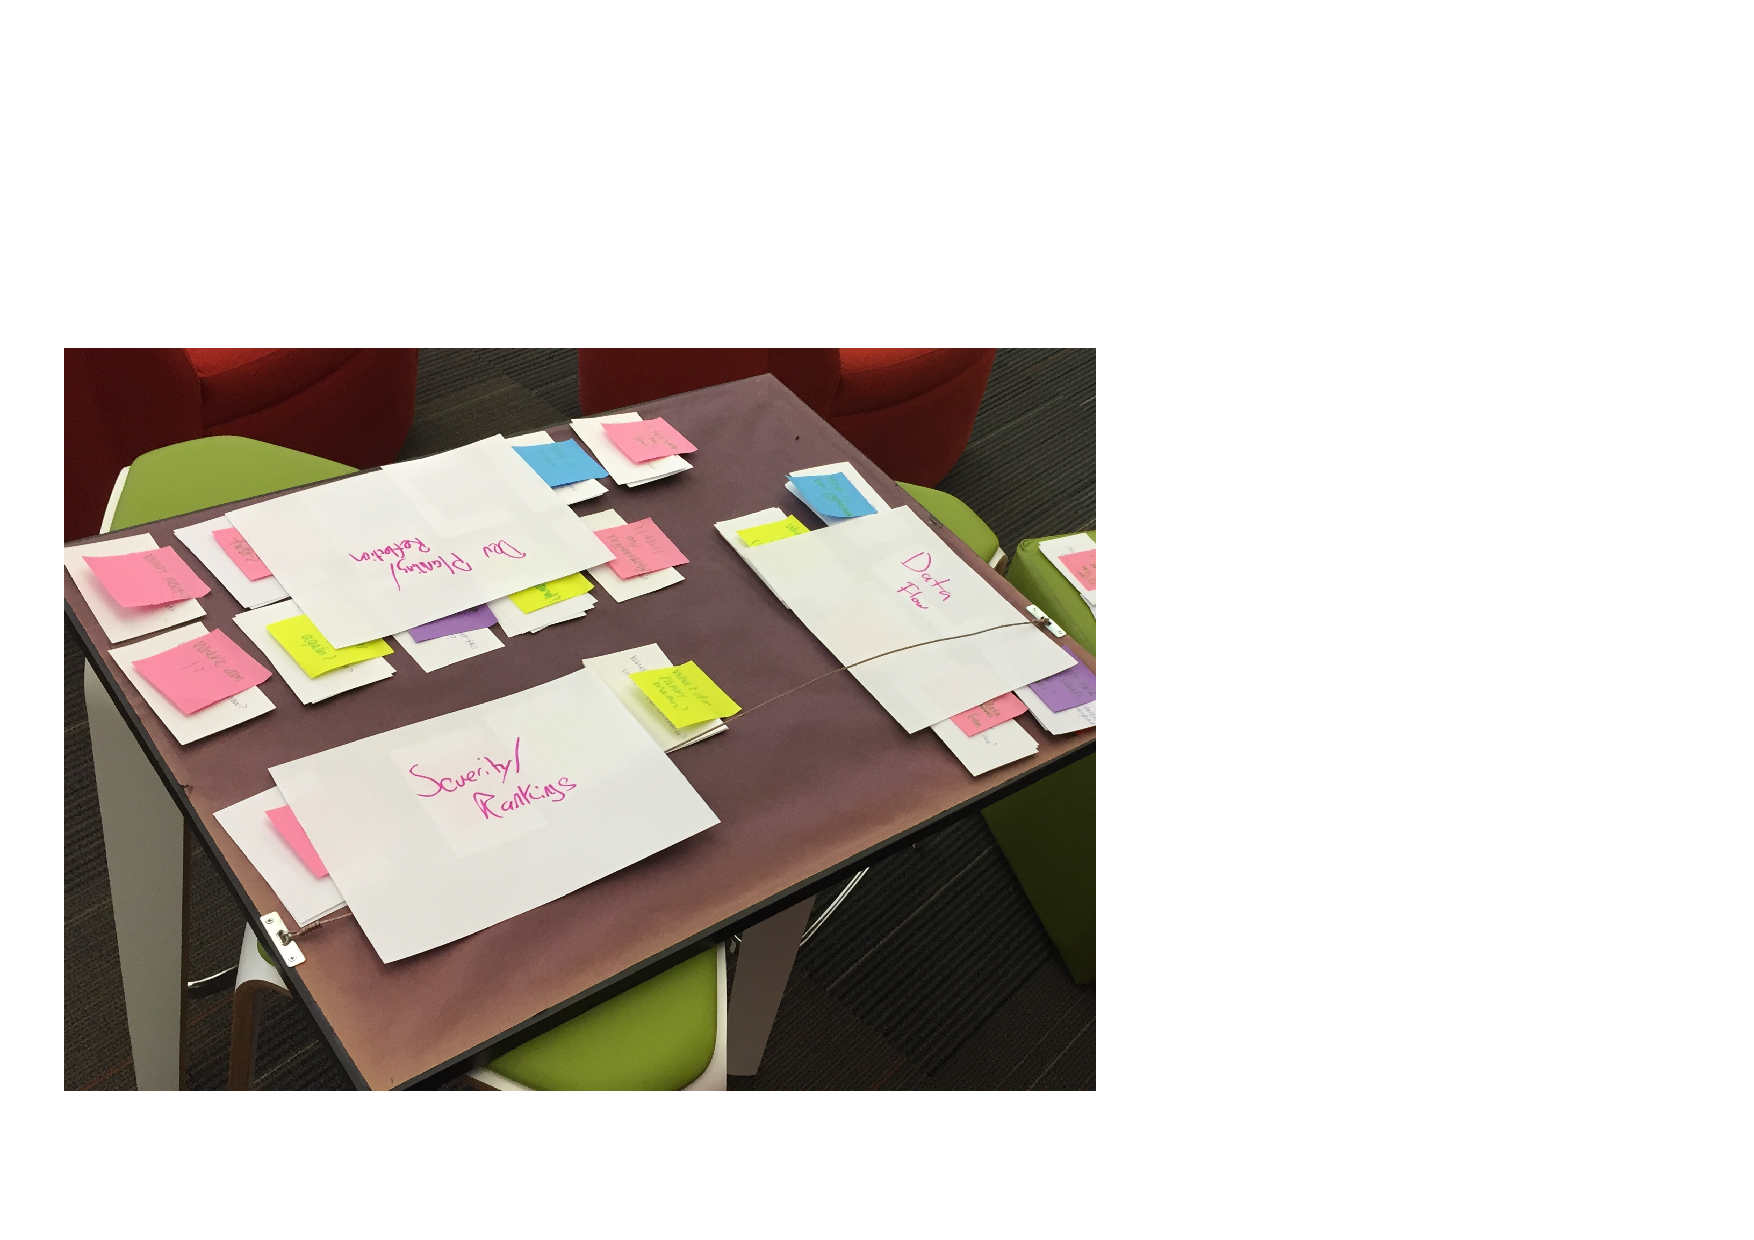
\includegraphics[width=3in]{Images/categories.pdf}
\caption{Sorting cards into categories based on emergent themes.}
\label{fig:cardsort} 
\end{figure}


\begin{table*} 
\centering
\caption{Emergent categories from card sort}
\begin{tabular}{|l|c|l|}
\rowcolor{gray!50}
\hline
    Category											& Count			& Example 	\\
    \hline		
    Developer Planning and Self-Reflection				& 14    		& \emph{Example question...}			\\
    \hline
    Bug Severity and Rank								& 4     		& \emph{Example question...}			\\
    \hline
    Data Storage and Flow								& 11     		& \emph{Example question...}		\\
    \hline
    Application Context/Usage							& 9     		& \emph{Example question...}			\\
    \hline
    Control Flow and Call Information					& 13     		& \emph{Example question...}		\\
    \hline
    Resources and Documentation							& 10     		& \emph{Example question...}			\\
    \hline
    Understanding and Interacting with Tools			& 9     		& \emph{Example question...}			\\
    \hline
    Understanding Alternative Fixes and Approaches		& 11     		& \emph{Example question...}			\\
    \hline
    Code Background and Function 	 					& 17     		& \emph{Example question...}			\\
    \hline
    Locating Information 								& 11      		& \emph{Example question...}			\\
    \hline
    Assessing the Application of the Fix				& 9     		& \emph{Example question...}			\\
    \hline
    Preventing and Understanding Potential Attacks		& 11     		& \emph{Example question...}			\\
    \hline
    Relationship Between Bugs							& 3     		& \emph{Example question...}			\\
    \hline
    End-User Interaction								& 3     		& \emph{Example question...}		\\
    \hline
    Error Messages										& 3     		& \emph{Example question...}			\\
    \hline
    Understanding Concepts								& 6 			& \emph{Example question...}				\\
    \hline
    Confirming Expectations					 			& 1				& \emph{Example question...}   \\
    \hline
    Uncategorized										& 10    		& \emph{} \\
    \hline
\end{tabular}
\label{table:categories}
\end{table*}


In the second stage, we identified emergent themes and grouped the clusters into categories based on the themes. 
For example, we placed the question \textit{Where can I get more information?} into a category called \emph{\textbf{Resources/Documentation}}, along with questions like \textit{Is this a reliable/trusted resource?} and \textit{What information is in the documentation}. 
Table~\ref{table:categories} contains the 17 categories along with the number of distinct clusters each contains. 

To validate the categories we identified, we asked two independent researchers to sort the question clusters into our categories. 
Rather than sort the entire set of questions, each rater was given a subset of the question set. 
The first rater agreed with our categorization with a Cohen's Kappa of $\kappa = .63$. 
Between the first and second rater we reworded and clarified some ambiguous questions. The second rater exhibited greater agreement ($\kappa = .70$). 
Given the high number of categories, these values are well within the acceptable ranges.

\section{Results}
\label{sec:results}
We list each distinct question we extracted and the count for each in parentheses. For each category, we discuss the common thread that ties questions in that category together. We also contextualize each category by discussing existing tool support and shortcomings.

\noindent\subsection{\textbf{Developer Planning and Self-Reflection (14)}} 

\noindent\emph{What was I looking for?} \\
\emph{What do I know now?} \\
\emph{What should I do first?} \\
\emph{Do I understand?} \\
\emph{Have I seen this before?} \\
\emph{What was that again?} \\
\emph{What's next?} \\
\emph{Where am I in the code?} \\
\emph{Is this worth my time?} \\
\emph{Is this my responsibility?} \\
\emph{Why do I care?} \\
\emph{Miscellaneous} \\

One kind of question participants asked when assessing potential security vulnerabilities in the code concerned their current status or plans for next steps in terms of understanding or assessing the vulnerability. Nine of the 155 distinct questions extracted fit into this category. All of the questions in this category involve the developer's thoughts or the individual's relationship to the problem, rather than specifics of the code or the error notification.  The most common occurring question in this category was...

Though these general questions may not be trivial to help developers answer, there may be ways to provide information or instructions developers can follow to more easily determine the answers for themselves. 
For example, one question participants asked was \textit{Have I seen this before?}
%Some participants described ad-hoc strategies for tracking the vulnerabilities they had encountered, such as keeping text files associated with 
A tool that helps developers answer this question might keep track of previous times the developer has encountered, and perhaps fixed, this vulnerability. 
The tool could also include a link to the code where the vulnerability was located as well as a diff showing the changes the developer made to fix the vulnerability.

%%%%%%%%%%%% Code Background

\noindent\subsection{\textbf{Code Background and Function (17)}}

\noindent\emph{Who wrote this code?} \\
\emph{Why is this code needed?} \\
\emph{Is this library code?} \\
\emph{Are there tests for this code?} \\
\emph{Why was this code written this way?} \\
\emph{What does this code do?} \\
\emph{Is this code doing anything?} \\
\emph{How much effort was put into this code?} \\
\emph{Why are we using this API in the code?} \\
\emph{Miscellaneous} \\

Participants also asked questions concerning the background and intended function of the code being analyzed. 
Nine of the 155 distinct questions extracted fit into this category. 
The questions in this category inquire about the code at an abstract level, such as determining the role a component or piece of code plays in the entire system or program.

The answer to many of these questions, developers would require aggregated data, such as documentation that programmers contribute to as the code changes or measuring the amount of effort that has been put into the code thus far.

This means that without proper tool support, developers interested in this information would have to seek out resources that have the information they need. Once they find the resource, they would have to find any and all information relevant to the program entity they are investigating, all while hoping the information is up to date and accurate. 


%%%%%%%%%%%% Locating Information

\noindent\subsection{\textbf{Locating Information (11)}}

\noindent\emph{Where is this used in the code?} \\
\emph{Where are other similar pieces of code?} \\
\emph{Where is this artifact?} \\
\emph{Is this artifact located in this class?} \\
\emph{Where is this method defined?} \\
\emph{Where is this class? } \\
\emph{Where is the next occurrence of this variable?} \\
\emph{How do I track this information in the code?} \\
\emph{How do I navigate to other open files?} \\
\emph{Miscellaneous} \\

Some participants asked questions regarding locating, or the ability to locate, information in their coding environment. 
Nine questions of the 155 extracted fit into this category.
The distinction between this category and \emph{\textbf{Code Background and Function}} is that this category includes questions pertaining to searches made in the coding environment for information, artifacts or code fragments. 
On the other hand, \emph{\textbf{Code Background and Function}} pertains to understanding the code at a higher level that would not be answered by triaging the code.

The answers to most of these questions can be found inside the IDE, which makes it more feasible for a tool to attempt to answer it. For example, Eclipse has an 'open declaration' tool that can be used to find a method's definition. A few of these questions, however, would require more effort on the developer's part to answer. For instance, it is not obvious how a tool would answer the question \emph{how do I track this information in the code}; the answer could vary depending on what information the developer is trying to track.


%%%%%%%%%%%% Assessing Application

\noindent\subsection{\textbf{Assessing the Application of the Fix (9)}}

\noindent\emph{How hard is it to apply a fix to this code?} \\
\emph{How do I use this fix in my code?} \\
\emph{How do I fix this vulnerability?} \\
\emph{Is there a quick fix for automatically applying a fix?} \\
\emph{Will the code work the same after I apply the fix?} \\
\emph{Can these fix suggestions be applied to my code?} \\
\emph{Will the error go away when I apply this fix?} \\
\emph{Does the code stand up to additional tests prior to/after applying the fix?} \\
\emph{What other changes do I need to make to apply this fix?} \\

Another kind of question we extracted pertained to the process resolving vulnerabilities. These questions pertain to understanding the application and implications of a potential fix. We categorized 9 of the 155 distinct questions into this category.

Though it is not clear how feasible it is to answer some of these questions, some can be answered by using a similar approach to that used by Mu{\c{s}}lu and colleagues when developing Quick Fix Scout~\cite{mucslu2012speculative}. 
Their tool attempts to help developers answer the question \textit{Does this fix introduce other bugs?} None of our participants asked this question specifically. 
However, questions like \textit{How hard is it to apply?} and \textit{Does the code stand up to additional tests prior to/after applying the fix?} could possibly be answered using a similar process.

  
%%%%%%%%%%%% Preventing and Understanding Potential Attacks 

\noindent\subsection{\textbf{Preventing and Understanding Potential Attacks (11)}}

\noindent\emph{How can this vulnerability lead to an attack?} \\
\emph{How can I replicate an attack that exploits this vulnerability?} \\
\emph{Why is this a vulnerability?} \\
\emph{What are the possible attacks that could occur?} \\
\emph{How can I prevent this attack?} \\
\emph{How should I address this problem? } \\
\emph{What is the problem (potential attack)?} \\
\emph{Is this a real vulnerability?} \\
\emph{How do I find out if this is a real vulnerability?} \\
\emph{Miscellaneous} \\

We also extracted questions pertaining to the potential attacks that could arise from the vulnerability found in the code. 
These questions aimed to understand the potential attacks that would exploit a given vulnerability, how to execute those attacks, how to prevent those attacks now and in the future. 
Nine of the 155 distinct questions we gathered belong in this category.

Some FindBugs notifications attempt to provide developers with the means to answer some of these questions by providing links to relevant information. 
Many of the links provided linked to information regarding why the code may be broken, however, do not provide information to improve understanding of what the potential attacks are.  

Some of the questions, such as \textit{how do I find out if this is a real vulnerability}, may not be as simple to answer by providing a link. 
This kind of question may require the triangulation of information; some information from the web on the vulnerability itself and the potential attacks, and some information from fellow developers who may better understand the likelihood the bug is a vulnerability. 
If there are resources, on the web or otherwise, that developers could use it does not seem that they are easy or intuitive to locate.


%%%%%%%%%%%% Control Flow/Call Information

\noindent\subsection{\textbf{Control Flow and Call Information (13)}}

\noindent\emph{What is the call hierarchy?} \\
\emph{How can I get calling information?} \\
\emph{Who can call this?} \\
\emph{Where is the method being called?} \\
\emph{What causes this to be called?} \\
\emph{Are all calls coming from the same class?} \\
\emph{What gets called when this method gets called?} \\
\emph{How often is this code called?} \\
\emph{Miscellaneous} \\

We also extracted questions relating to control flow and calling information. 
Developers seek information information pertaining to the methods that get called, or do not get called, in the code. 
As the name of this category suggests, these questions can generally be answered using a tool for viewing the call hierarchy, when available. 
Eight of the 155 distinct questions extracted dealt with acquiring control flow and call information.

%EXPAND ON CALL HIERARCHY TOOL
Eclipse includes a call hierarchy tool that, given a method, displays its callers and all its callees. 
The tool allows users to easily traverse the call hierarchy. 
While some participants located and employed the call hierarchy tool, others gravitated toward other more error-prone approaches, such as the 'find references' tool or manual visual inspection. 
%find references / visual inspection
In some cases, participants were unaware of the call hierarchy tool or how to use it. Others were predisposed to favor light-weight tools, such as inspecting code highlights, rather than navigate to and invoke the call hierarchy tool.
It is unclear whether the call hierarchy tool is more efficient than tools like 'find references' for answering these kinds of questions, however participants who sought call information without the call hierarchy tool were more likely to make faulty assumptions or miss method calls. 
Even with tools like these, however, it may be difficult to easily/quickly answer questions like \emph{how can I get calling information} and \emph{who can call this} without having to manually, and mentally, aggregate the information gathered from each tool. 
Further, even tools like call hierarchy do not provide information on how parameters are modified between method calls.


%%%%%%%%%%%% Data Storage 

\noindent\subsection{\textbf{Data Storage and Flow (11)}}

\noindent\emph{How is data put into this variable?} \\
\emph{Does data from this method/code travel to the database?} \\
\emph{Where does this information/data go?} \\
\emph{How do I find where the information travels?} \\
\emph{How does the information change as it travels through the programs?} \\
\emph{What does the variable contain?} \\
\emph{Is any of the data malicious?} \\
\emph{Where is the data coming from?} \\
\emph{Miscellaneous} \\

Some of the questions we found pertained to the data being stored and carried throughout the program. 
Often participants wanted to understand  the type of data being collected and stored, where the data came from, and where it was going. 
Eight of the 155 distinct questions fit into this category.

The call hierarchy tool in Eclipse provides a way of understanding control flow, but this static information does not give an idea of how data travels when the program is run. 
The developer would have to retrieve this information, either from the documentation, by debugging the code, or some combination of both. 
There exists tools that do data flow analysis and report defects to programmers based on said analysis, however, they do not allow developers to explore the flow of data through their programs~\cite{jovanovic2006pixy}. 
There has been some research and development surrounding the creation of data flow graphs for visualizing data dependencies in a program, however, data dependency graphs become unwieldy as applications grow large~\cite{ghosh2001method, ferrante1987program}.
% tools that do data flow analysis (i.e. Pixy) but do not allow developer to explore the flow of data.


%%%%%%%%%%%% Application Context

\noindent\subsection{\textbf{Application Context/Usage (9)}}

\noindent\emph{What is the method/variable used for in the program?} \\
\emph{Are we handling secure data in this context?} \\
\emph{What is the context of this bug/code?} \\
\emph{How does the system work?} \\
\emph{Will usage of this method change?} \\
\emph{Is the method/variable every being used?} \\
\emph{Is this code used to test the program/functionality?} \\
\emph{Miscellaneous} \\

Some participants wanted to know how code entities or pieces of code fit into the overall context of the application or system under analysis. 
The questions ranged from specific questions about a method or variable to general questions regarding the usage of the entire system. 
Seven of the 155 distinct questions revolved around how the code works in the context of a portion of or the entire system.

%FAMILIARITY

Though all participants had experience coding in iTrust, and had some knowledge about the codebase, many still encountered situations where they wanted to know the usage or context of a segment of code within the application. 
It is not obvious what tool support for answering these kinds of questions would look like, especially when it is not obvious why participants wanted these bits of information. 
For example, one reason for needing this type of information is to better understand the code and likelihood that a bug is a vulnerability. However, it may be that participants merely wanted to know the answers to these questions with no high level goal in mind.

%%%%%%%%%%%% Resources

\noindent\subsection{\textbf{Resources and Documentation (10)}}

\noindent\emph{What type of information does this resource link me to?} \\
\emph{What is the documentation?} \\
\emph{Can my team members/resources provide me with more information?} \\
\emph{Where can I get more information?} \\
\emph{What information is in the documentation?} \\
\emph{Is this a reliable/trusted resource?} \\
\emph{How do resources prevent or resolve this?} \\
\emph{Miscellaneous} \\

Another kind of question we extracted pertained to the resources and documentation available regarding the vulnerability or source code. 
Many participants found themselves in situations where they would use outside resources to decide how to proceed. 
Seven of the 155 distinct questions fall into this category. 

%Fix Sentence
Some tools link to external documentation that developers can use to attempt to answer some of these questions, Find Security Bugs being one of them. 
Though links to external documentation and resources can provide answers to some of these questions, they do not help answer questions concerning the reliability of the resource nor do they provide developers with the ability to locate and use other external resources such as team members or others who have experience with the relevant code.
%Information too complex, not sure how to apply 
Lack of support for answering these questions may have contributed to participants not clicking the links in many situations.  
Fritz and colleagues developed a degree of knowledge model that predicts how familiar a developer is with various source code elements, however, this model has not been operationalized in a tool that allows developers to have access to the degree of knowledge values for various developers on the code segment being analyzed~\cite{fritz2010degree}.


%%%%%%%%%%%% Understanding Interacting Tools

\noindent\subsection{\textbf{Understanding and Interacting with Tools (9)}}

\noindent\emph{Why is the tool complaining?} \\
\emph{What is the tool output telling me?} \\
\emph{Can I verify the information the tool provides?} \\
\emph{What is the tool keybinding?} \\
\emph{What is the tool's confidence?} \\
\emph{What tool do I need for this?} \\
\emph{How is the information presented by the tool organized?} \\
\emph{Miscellaneous} \\

Throughout the study participants interacted with a variety of tools including Find Security Bugs, the call hierarchy tool, and find references, for example. 
While interacting with these tools, participants asked questions about how to access specific tools and how to interpret their output. 
Seven of the 155 distinct questions we extracted fall into this category.

%[ACCESSIBILITY (4 letter word)]
Some of the questions we extracted seemed to deal with having access to or knowing how to use the tools needed to complete a certain task. 
Participants sometimes found themselves in situations where they needed information or to take action but could not determine how to invoke the tool or possibly did not know what tool they would use at all. 
This seems to point to a tool awareness or education problem.


%[Presentation of tool information]
Other questions dealt with the presentation of information provided by the tool. 
Participants wanted to be able to explore things about the tool's output, and typically had to manually determine the answers to their questions. 
For example, Find Security Bugs reports its confidence on the potential defect in the notification, however, some participants found it difficult to process this information.



%%%%%%%%%%%% Understanding Alt. Fixes

\noindent\subsection{\textbf{Understanding Alternative Fixes and Approaches (11)}}

\noindent\emph{Why should I use this alternative method/approach to fix the vulnerability?} \\
\emph{What are the alternatives for fixing this?} \\
\emph{Does the alternative function the same as what I'm currently using?} \\
\emph{When should I use the alternative?} \\
\emph{Is the alternative slower?} \\
\emph{Are there other considerations to make when using the alternative(s)?} \\
\emph{How does my code compare to the alternative code in the example I found?} \\
\emph{Miscellaneous} \\

Sometimes participants looked elsewhere for information about their code or vulnerability. 
Primarily, participants used web resources or searched for similar code elsewhere in the project.
When presented with alternative approaches or solutions, participants compared the alternative with the current code and assessed the applicability of the alternative. 
Seven of the 155 questions we extracted pertained to understanding the various facets of alternative approaches or solutions.

The process of understanding the alternative options was complicated by the variety of sources, such as StackOverflow, official documentation, and personal blogs, that all presented information in different formats.  
Often the candidate alternative did not readily provide meta-information about trade-offs or the process of applying suggestions. 
Many participants seemed to have a preference for StackOverflow as a means for understanding alternative approaches and fixes. 
%%%%%%%%%%%% Bug Severity/Ranking

\noindent\subsection{\textbf{Bug Severity and Ranking (4)}}

\noindent\emph{How serious is this bug?} \\
\emph{Are all these bugs the same severity?} \\
\emph{How do the rankings compare?} \\
\emph{What do the bug rankings mean?} \\

Some participants had questions regarding the severity or ranking of the bug being reported by FindBugs. 
These questions dealt with general bug severity questions or severity and ranking questions pertaining specifically to the tool and how it categorizes/groups bugs. 
Four of the 155 distinct questions extracted fall into this category. 
Previous research on static analysis tools also found that developers may not always be able to understand the rankings or severity labels tools use, so it is not surprising this category emerged from our questions~\cite{johnson2013don}.

%%%%%%%%%%%% Relationship Between Bugs

\noindent\subsection{\textbf{Relationship Between Bugs (3)}}

\noindent\emph{Does this other piece code have the same bug as the code I'm working with?} \\
\emph{Are all the bugs related in my code?} \\
\emph{Are all of these notifications vulnerabilities?} \\

Some participants asked questions about the connections between co-occurring vulnerabilities and whether or not similar vulnerabilities exist elsewhere in the code. 
Three of the 155 distinct questions we found target the relationships between the vulnerabilities in the code. 
We speculate that developers might have these kinds of questions because they want to know if a vulnerability like the one they are assessing exists in other similar code fragments. 
Another reason for asking this kind of question is to determine the possibility of eliminating more than one vulnerability with one fix. 
Whatever the motivation may be, participants did not seem to have an intuitive or easy way of going about finding the answer to the questions asked in this category.
%%%%%%%%%%%% End-User Interaction

\noindent\subsection{\textbf{End-User Interaction (3)}}

\noindent\emph{Is there input coming from the user?} \\
\emph{Does the user have access to this code?} \\
\emph{Does user input get validated/sanitized?} \\

Questions in this category deal with how the end user might interact with the system. 
Participants wanted to know whether users could access critical parts of the code and if measures are being taken to mitigate potential malicious activity. 
Three of the 155 distinct questions we found fall into this category.

Research exists that studies attack surfaces, or vectors that predict where an unauthorized user may be able to gain access to the system. 
The goal of this research area is to identify, measure, and reduce the size of attack surfaces~\cite{manadhata2011attack, bartel2012automatically}. 
To our knowledge, developers lack tool support for navigating and reasoning about attack surfaces. 
Many participants spent time and effort exploring the call hierarchy of the potential path traversal only to discover that the code was entirely contained in test classes.
 
%%%%%%%%%%%% Understanding Concepts

\noindent\subsection{\textbf{Understanding Concepts (6)}}

\noindent\emph{What is the term for this concept?} \\
\emph{Do these words have special meaning related to this concept/problem?} \\
\emph{How does this concept work?} \\
\emph{What is this concept?} \\
\emph{Miscellaneous} \\

For some participants, the concepts that the notification contained were incompatible with the developer's mental model. 
In these situations, participants seemed to have questions surrounding one or more of the concepts relevant to the problem.

Sometimes, the difficulty participants encountered was with the terminology used; others were not familiar with some of the general concepts being discussed. 
In general, it seems that if a developer does not have experience with a particular feature or concept, it is less likely they will understand a problem in their code pertaining to that concept~\cite{}.%cite building mental model paper? 
%%%%%%%%%%%% Confirming Expectations

\noindent\subsection{\textbf{Confirming Expectations (1)}}

\noindent\emph{Is this doing what I expect it to?} \\
%Swap categories?
Developers build and alter their mental models when exploring code~\cite{canas1994mental, burkhardt1997mental}. 
As they build and alter mental models, developers may seek confirmation that they fully understand the code and its intended function; for a subset of our participants, this was the case. 
We only identified one distinct question, however, there are many ways to interpret the questions and may require different pieces of information to answer it.

%%%%%%%%%%%% Error Messages

\noindent\subsection{\textbf{Error Messages (3)}}

\noindent\emph{What is the relationship between the error message and the code?} \\
\emph{What code caused this error message to occur?} \\
\emph{What does the error message say?} \\

As expected, participants asked questions concerning the content of the error messages. 
Mostly, this happened when participants needed to look at the bug information to get a better understanding of the potential vulnerability. 

More surprisingly, they also asked questions about how to relate information contained in the error message back to the code. 
For example, the predictable random vulnerability notes that a predicable random value is bad when being used in a secure context. 
Many participants attempted to related this piece of information back to the code by looking to see if anything about the code where the potential vulnerability was found suggests it is in a secure context. 
In this situation, the fact that the method the vulnerability was found in was called \texttt{randomPassword()} suggested to participants that the code was in a secure context and therefore a vulnerability that should be resolved.

\section{Discussion}
\label{sec:disc}
Data suggests that tools should focus on XYZ. Discuss interesting/contradictory categories and implications.

COME UP WITH SECTION HEADERS

%Whyline, flow of data and control

\section{Future Work}
\label{sec:fw}

\section{Conclusion}
\label{sec:concl}
The conclusion goes here.




% conference papers do not normally have an appendix


% use section* for acknowledgement
\section*{Acknowledgment}


The authors would like to thank...


\bibliographystyle{IEEEtran}
% argument is your BibTeX string definitions and bibliography database(s)
\bibliography{iTrustInterviews}
%
% <OR> manually copy in the resultant .bbl file
% set second argument of \begin to the number of references
% (used to reserve space for the reference number labels box)




% that's all folks
\end{document}


